\documentclass[10pt, a4paper]{article}
\usepackage[utf8]{inputenc}
\usepackage[T1]{fontenc,url}
\usepackage{multicol}
\usepackage{multirow}
\usepackage{parskip}
\usepackage{lmodern}
\usepackage{microtype}
\usepackage{verbatim}
\usepackage{amsmath, amssymb}
\usepackage{tikz}
\usepackage{physics}
\usepackage{mathtools}
\usepackage{algorithm}
\usepackage{algpseudocode}
\usepackage{listings}
\usepackage{enumerate}
\usepackage{graphicx}
\usepackage{float}
\usepackage{hyperref}
\usepackage{tabularx}
\usepackage{siunitx}
\usepackage{fancyvrb}
%\usepackage{natbib}
%\bibliographystyle{dinat}
\usepackage[makeroom]{cancel}
\usepackage[margin=1.4cm]{geometry}
\usepackage{pdfpages}
\usepackage[margin=10pt, textfont={small, it}, labelfont={bf}, labelsep=endash]{caption}
\renewcommand{\baselinestretch}{1}

\begin{document}
\title{COMAP - Vane angle analysis}
\author{
    \begin{tabular}{r l}
        Jonas Gahr Sturtzel Lunde & (\texttt{jonassl@astro.uio.no})
    \end{tabular}}
% \date{}    % if commented out, the date is set to the current date
\maketitle
Relevant code found at \url{https://github.com/jgslunde/comap_general/tree/master/vane_angle}
\vspace{0.7cm}


\renewcommand{\abstractname}{Summary}
\begin{abstract}
    \noindent
    This write-up summarizes an effort to analyze the behavior and relation of the COMAP telescope feedhorn array and the angle of the calibration vane, with the goal of finding a suitable "safe" threshold angle of the vane for a successful $T_{sys}$ measurements. By interpolating the spectrometer TOD power data onto the vane angle data, we study the relation between two. Additionally, the minimum obtainable angle, and frequency of stuck vane states were analyzed, to assert the health of the calibration vane. \\
    
    \noindent
    We found that the interpolation produces inconsistent results, which can only be explained by an erroneous offset in the timestamps reported by the spectrometer. This offset was found to be a delay of $\sim 0.6$ seconds. Correcting for this delay, we found that a threshold angle of $68$ degrees is sufficient for good $T_{sys}$ measurements, as the signal in feeds 8 and 10 falls by $1\%$ already at a vane angle of $68.88$ degrees. Additionally, we discovered that the minimum angle obtainable by the calibration vane suddenly increased from an average of $65.5$ degrees to $66.1$ degrees, combined with a much larger spread in values from obsid to obsid. This transition to a higher, more scattered minimum angle state happened sometime around obsid $9730$, MJD $58830$ (2019-12-13). Lastly we found a large increase in the number of stuck vane states from obsid ca. 13000-13500 and onward. 
\end{abstract}




\section{Introduction}
The $T_{sys}$ calibration of the telescope involves tilting a calibration vane across the telescope receiver. As each of the 19 feedhorns in the receiver array gets gradually covered, their TOD signal will spike. The vanes position is defined by an angle, which takes a value of $\sim 220$ degrees when the vane is idle, and $\sim 66$ degrees when it completely covers the array.

A good $T_{sys}$ measurement requires confidence that all feeds are comfortably covered by the vane. Due to the physical layout of the feeds, we expect their spikes in signal to come at different vane angles. The goal of this writeup is to identify at what vane angle a $T_{sys}$ measurement can be made with confidence.


\section{Implementation}
We will be using the TOD signal data found in the \texttt{/spectrometer/tod} dataset of the level1 files, combined with the timestamps in \texttt{/spectrometer/MJD}. The vane angles are found in \texttt{/hk/antenna0/vane/angle}, coupled with the timestamps from \texttt{/hk/antenna0/vane/utc}\footnote{Despite the confusing name, these timestamps are all in MJD.}. Finally, the information about the state of the array (like "doing $T_{sys}$ calibration") is found in \texttt{/hk/array/frame/features}, together with timestamps in \texttt{/hk/array/frame/utc}. We will in practice assume that the antenna0 and array timestamps are identical, using only the antenna0 one for both arrays. This turns out to be a fine assumption. They have the time timeintervals between timestamps, and a slight (subsecond) offset in their values. This doesn't matter, as it is the angle which gets us our final results, and the array state is simply used to discards parts of the dataset where no $T_{sys}$ measurements are taken.


\section{First look}
Figure \ref{fig:tod_angle} shows four randomly selected $T_{sys}$ measurements, gathered from level1 files. We can see the vane angle decreases to $\sim 66$, and the power in all feeds spike as the angle approaches its minimum, although at slightly different times for each feed, as expected.

\subsection{Time offset problem}
A worrisome observation is that the the spike in power does not appear completely symmetric with the fall and rise in vane angle. One would expect the power of each feed to be unique for any given vane angle. In other words, we would expect the power to be the same value as the vane passes, say, 100 degrees, independently of whether this angle appears while its descending or ascending. This does not appear to be the case, and the TOD power seems to be lagging slightly behind the vane angles.

Figure \ref{fig:tod_angle_scatter} shows this problem even more clearly. Here, all available vane angles for $T_{sys}$ measurements of 2019-07 through 2020-06 are gathered, with TOD power interpolated onto the reported vane angle timestamps. What we expect is a single logistic-looking curve, with power $1$ at very low angles, power $\sim 0$ at very high angles, and a logistic-looking transition in between. Instead, we get two such curves. It seems clear that one of these curves are from the descension of the vane, and one is from the following ascension of the vane, which should in theory overlap, but does not.

\begin{figure}[H]
    \centering
    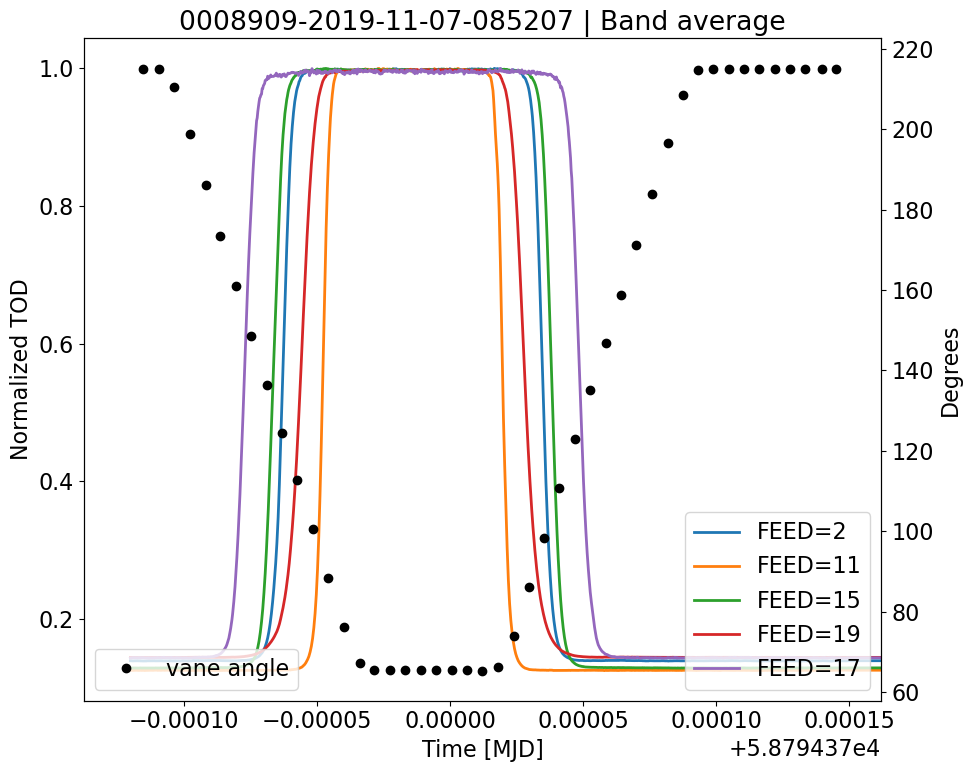
\includegraphics[scale=0.34]{../plots/tod_angle_0008909-2019-11-07-085207.png}
    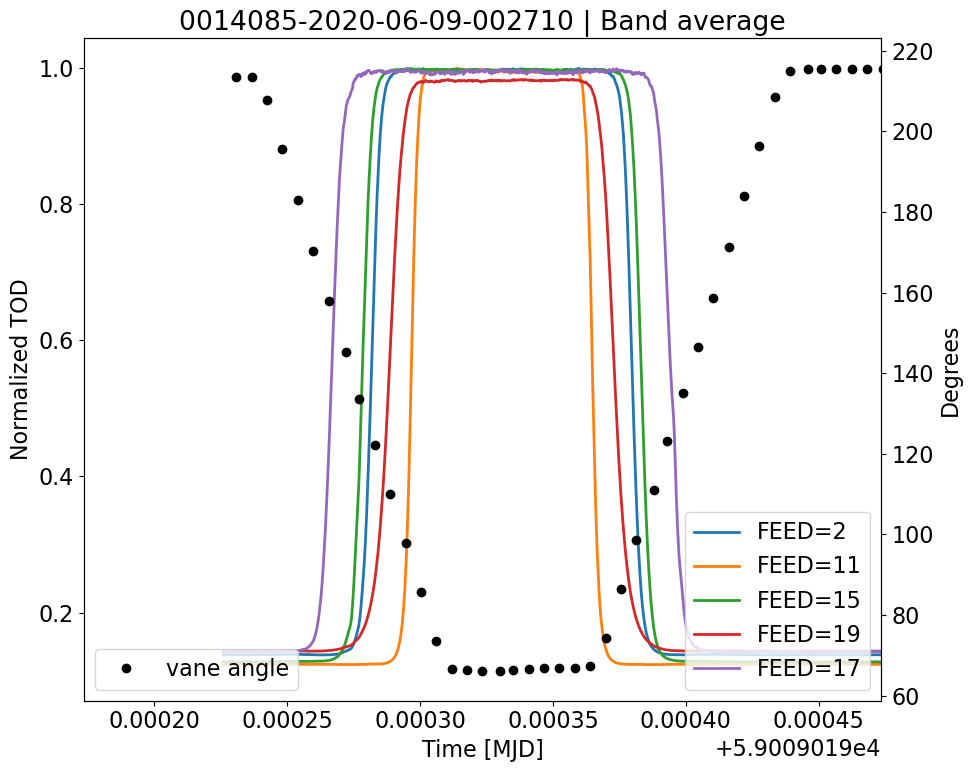
\includegraphics[scale=0.34]{../plots/tod_angle_0014085-2020-06-09-002710.png}
    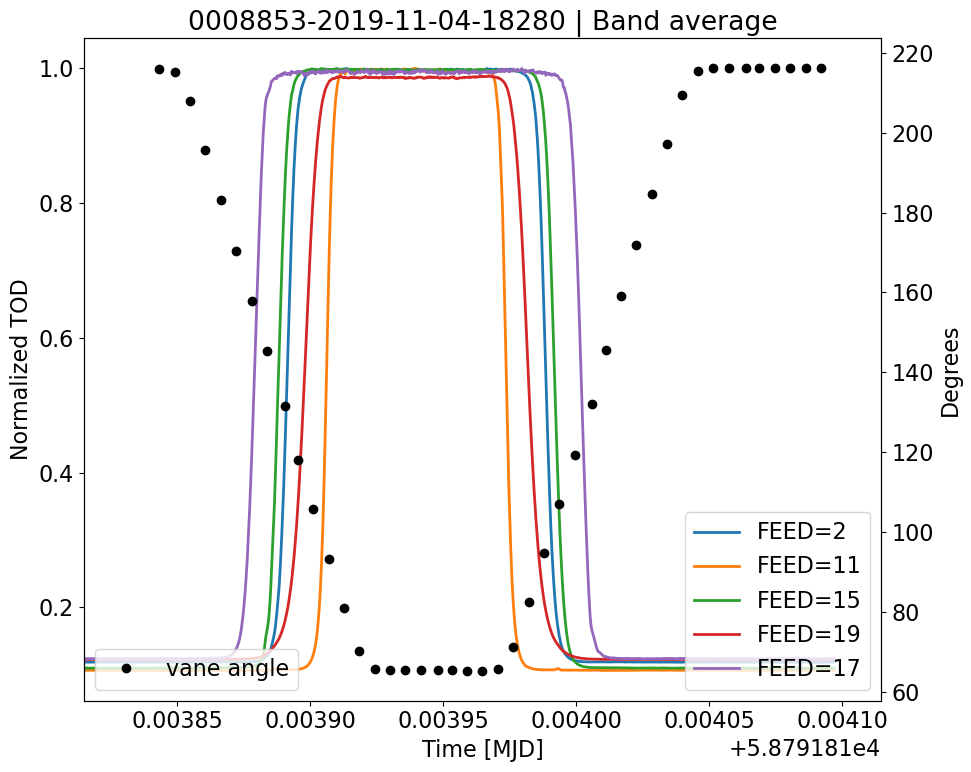
\includegraphics[scale=0.34]{../plots/tod_angle_0008853-2019-11-04-18280.png}
    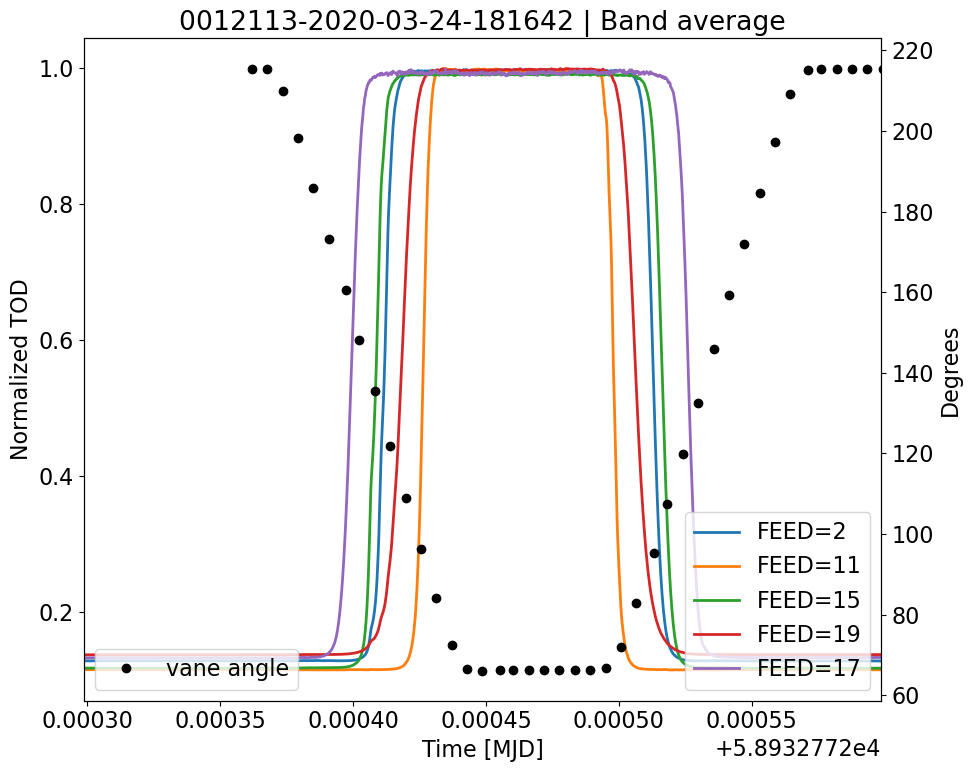
\includegraphics[scale=0.34]{../plots/tod_angle_0012113-2020-03-24-181642.png}
    \caption{Normalized TOD power (thin lines) for a handful of feeds of four random level 1 files, together with vane angle (black dots) for four Tsys measurements. The TOD/angle relation should be completely symmetric in time, but a light offset can be seen (the TOD is seemingly lagging behind the vane angle). Another (expected) observed effect is the different widths of each feeds TOD power curve, due to their differing physical placements on the feed array.}
    \label{fig:tod_angle}
\end{figure}

\begin{figure}[H]
    \centering
    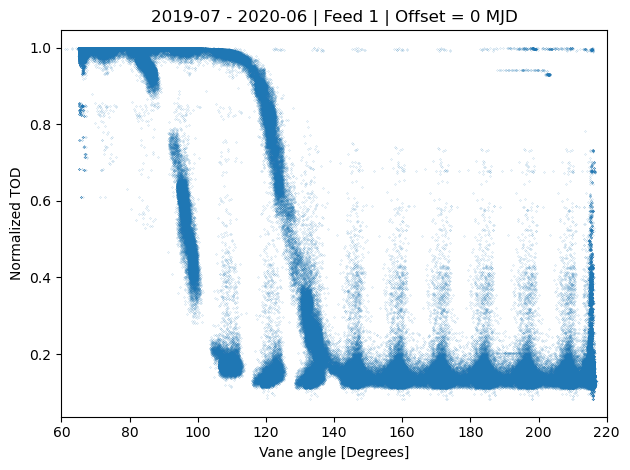
\includegraphics[scale=0.6]{../plots/power_angle_all_0.png}
    \caption{Normalized TOD vs vane angle for feed 1. Each dot represents a single reported vane angle, with a TOD power interpolated onto it. The plot contains all functional level 1 files for 12 months. We would expect the TOD/vane relation to be consistent between "vane descending" and "vane ascending", but we see two very distinct TOD/angle curves. This suggests an offset between the TOD and angle timestamps.}
    \label{fig:tod_angle_scatter}
\end{figure}



\subsection{Temporary solution to time offset problem}
Since we know what we want the power/angle curve to look like, we can temporarily overcome this issue by introducing an offset in the timestamps reported by the spectrometer until the curves fall on top of each other. Some trail and error produced the curve seen in figure \ref{fig:tod_angle_scatter_offset}, which is how we expect it too look. This required an offset of $7\times 10^{-6}\,\si{MJD} \approx \SI{0.6}{s}$.

To get an idea of the size of this offset compared to the different time intervals used by the telescope, figure \ref{fig:time} shows the 0.6 second offset against the first 10 (top) and 1 (bottom) seconds of timestamps from the spectrometer, antenna0, and array. The offset is slightly longer than a single timestamp in the antenna or array, which both have timesteps of $\sim 0.5$ seconds, while being significantly longer than a timestamp in the spectrometer. Since it is the spectrometer which appears to lags behind, it is surprising to see that the offset is instead of the order of magnitude of the antenna and array. It is also slightly frustrating that, while it is indeed of the order of one anbtenna or array timestep, it is undoubtedly somewhat larger (0.6 vs 0.5 seconds), ruling out a simple index bug in someones code.

Another observation is the fact that the timestamps don't start at the exact same time. As a matter of fact, the antennas first timestamp is a fraction of a second behind the first spectrometer timestep, and the first array timestep is almost 0.5 seconds behind. It is unclear to me why the antenna and array timestamps line up so poorly, especially considering they seem to contain cross-relevant information (the vane "state", e.g. "doing a Tsys measurements" is in the array container, while the actual vane angles lie in the anteanna0 container).

\begin{figure}[H]
    \centering
    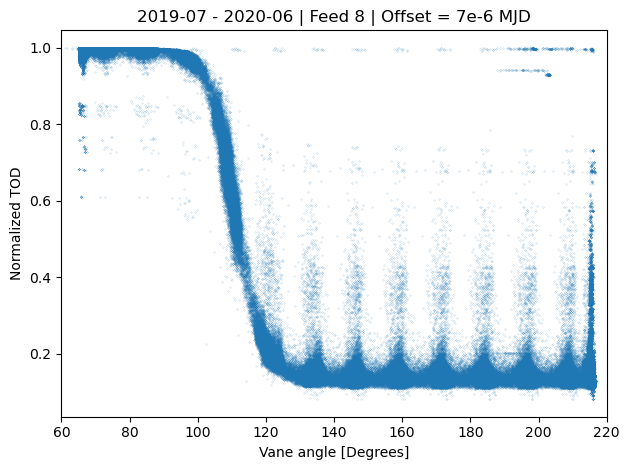
\includegraphics[scale=0.6]{../plots/power_angle_all_7e-6.png}
    \caption{Same plot as figure \ref{fig:tod_angle_scatter}, but with a delay of 7e-6 MJD (0.6 seconds) introduced to the TOD power before doing the interpolation. This delay gives us the plot like we expect it to look.}
    \label{fig:tod_angle_scatter_offset}
\end{figure}


\begin{figure}[H]
    \centering
    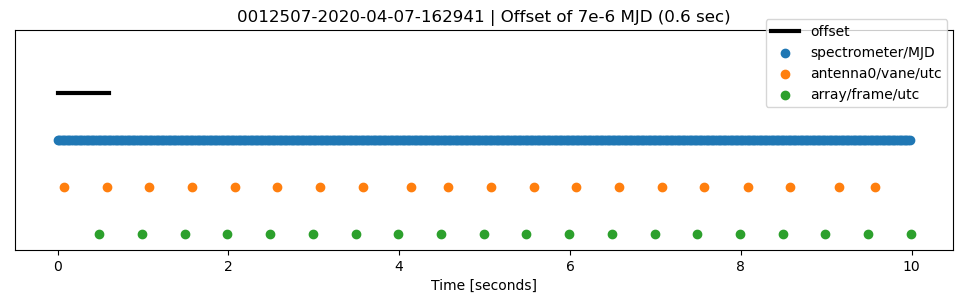
\includegraphics[scale=0.5]{../plots/times_20.png}
    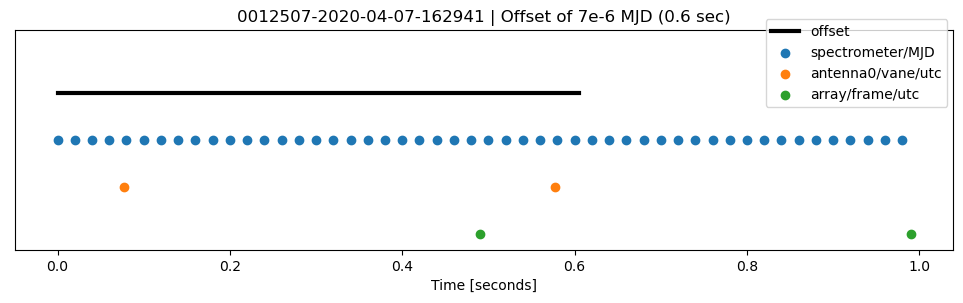
\includegraphics[scale=0.5]{../plots/times_2.png}
    \caption{Plots showing the first 10 (top) and 1 (bottom) seconds of time stamps of the TOD, antenna0, and array. The offset we had to be introduced to get consistent results in previous plots is also shown, as a black line. All timestamps are subtracted the first value of the spectrometer timestamps, which had the earliest timestamp of the three.}
    \label{fig:time}
\end{figure}




\section{Finding vane angle threshold}
\subsection{Overview}
Equipped with our improvised solution to the time offset problem, we can get back to actually estimating the optimal vane angle for good $T_{sys}$ measurements. Expanding on figure \ref{fig:tod_angle_scatter_offset}, the same 12-month data was binned in 0.25 degree bins (using simply the average value) for each feed, and plotted in figure \ref{fig:binned_all}. As we can see, there is a huge difference in at what angle different feeds lose power. The "worst" feeds are without a doubt feed 8 and 10, with 9 right behind. This is due to their physical placement furthest away from the calibration vane. Figure \ref{fig:layout} shows at what angle each feed falls in power by $2.5\%$, depending on their physical placement. 

\vspace{1cm}
\begin{figure}[H]
    \centering
    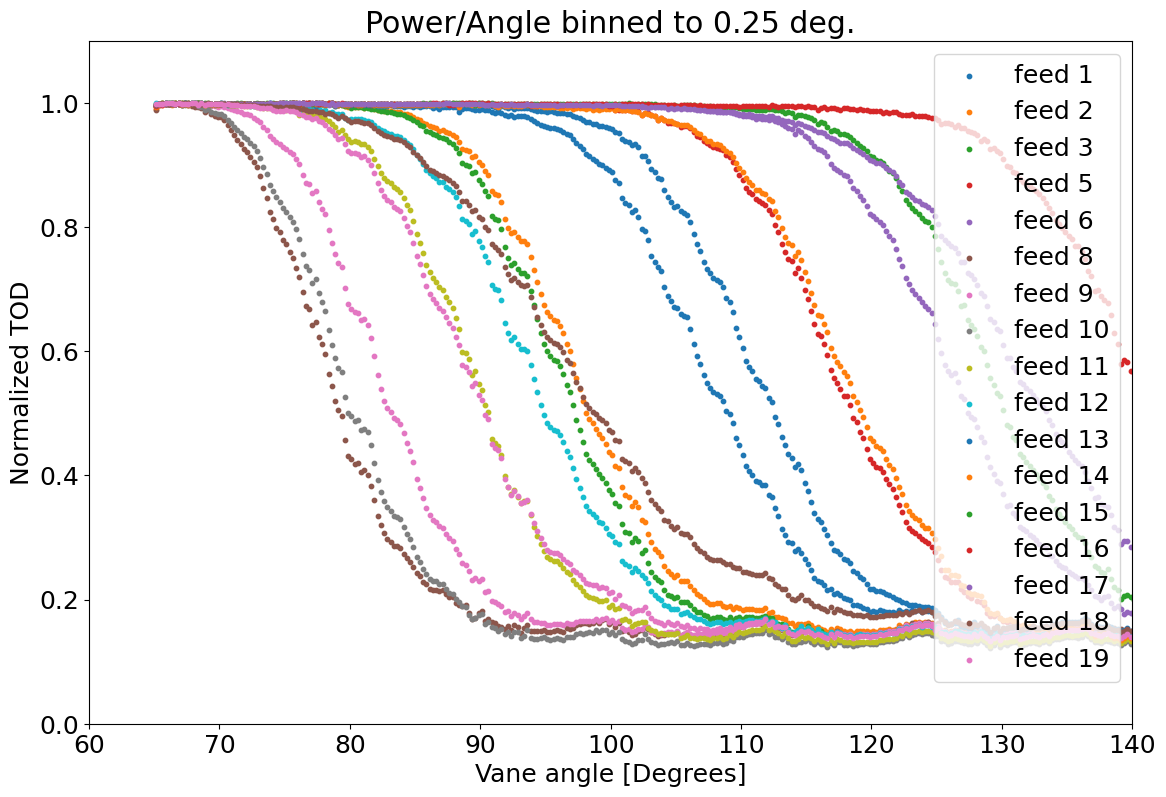
\includegraphics[scale=0.4]{../plots/binned_all.png}
    \caption{Scatter plot showing the power/angle relation of the calibration vane for all feeds, binned to 0.25 degrees. 12 months of level 1 files, from 2019-07 through 2020-06 was used.}
    \label{fig:binned_all}
\end{figure}


\vspace{1cm}
\begin{figure}[H]
    \centering
    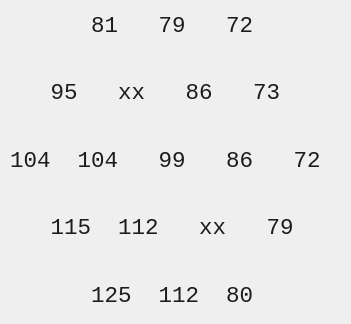
\includegraphics[scale=0.5]{../plots/vane_nums1.png}
    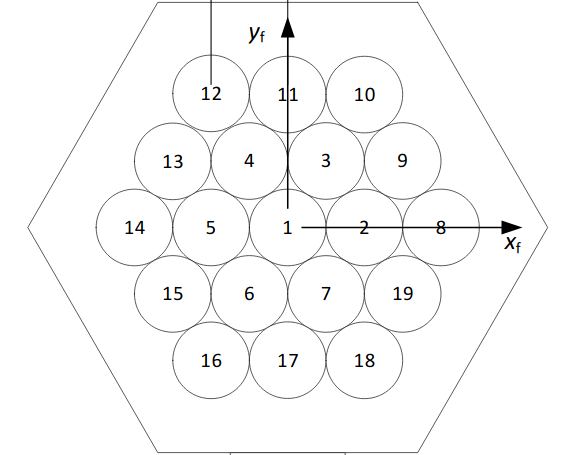
\includegraphics[scale=0.4]{../plots/vane_nums2.png}
    \caption{Angles for which the different feeds pass below the 97.5\% power threshold, ordered after their physical placement on the array.}
    \label{fig:layout}
\end{figure}



\subsection{Analysis of feed 8 and 10}
The two worst feeds (meaning the last to gain power when the calibration vane decreases in angle) are feeds 8 and 10. We will therefore use these two as a baseline when picking an optimal angle for $T_{sys}$ measurements. Figure \ref{fig:8and10} shows a zoomed in version of figure \ref{fig:binned_all} on the two feeds. Markers at $1\%$ and $2\%$ fall in power, and errorbars, are also included. As we can see, both feeds have lost $1\%$ power at $66.88$ degrees. It does appear that the power starts decreasing every so slightly from about $68$ degrees and onward.

This view is further supported up by figure \ref{fig:8and10_diff}, which shows the difference between each bin and the former. If these points are consistently below zero, we have a negative derivative, and a systematic decrease in power. The points are comfortably close to zero all the way to somewhere around $68$ - $68.5$ degrees, at which point they not only start decreasing, but also contain a much larger spread. 


\vspace{1cm}
\begin{figure}[H]
    \centering
    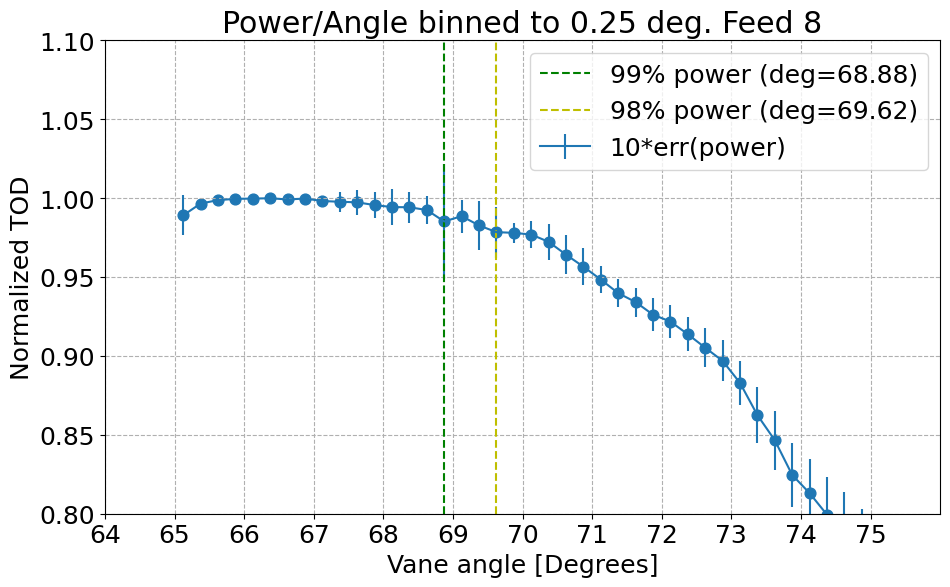
\includegraphics[scale=0.36]{../plots/binned8.png}
    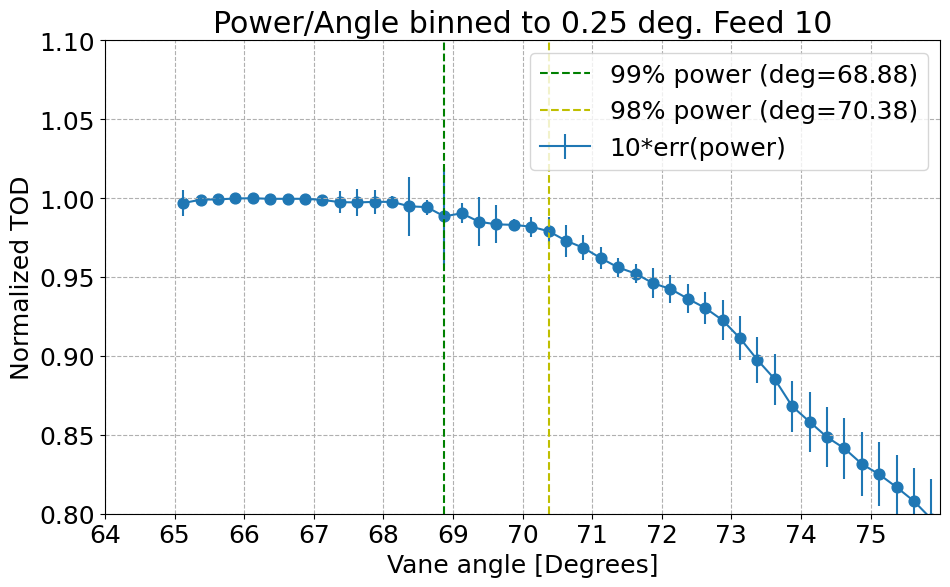
\includegraphics[scale=0.36]{../plots/binned10.png}
    \caption{Scatter plot showing the power/angle relation of the calibration vane for the three "worst" feeds, binned to 0.25 degrees. Error bars show $\sigma(x)/\sqrt{N}$, magnified by a power of 10, for clarity.}
    \label{fig:8and10}
\end{figure}

\vspace{1cm}
\begin{figure}[H]
    \centering
    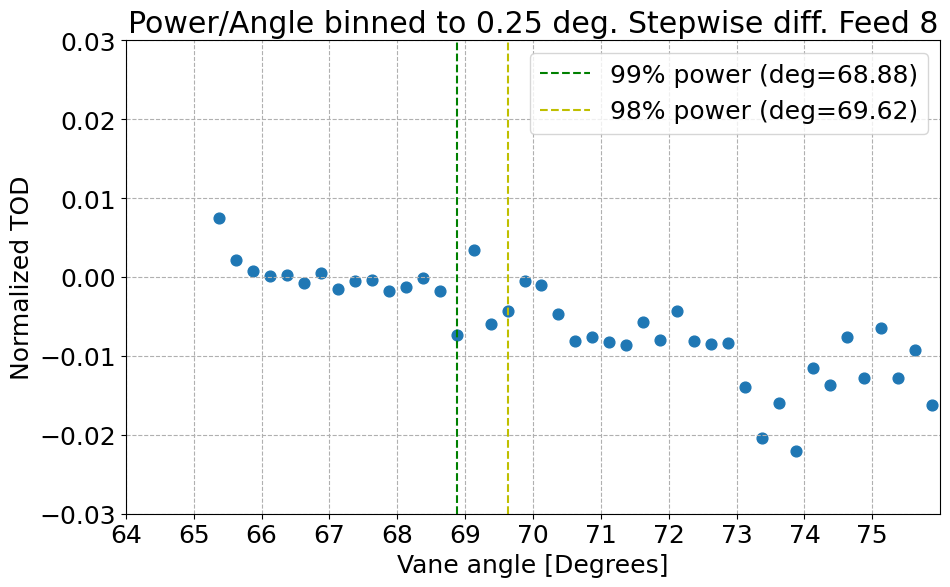
\includegraphics[scale=0.37]{../plots/binned_diff8.png}
    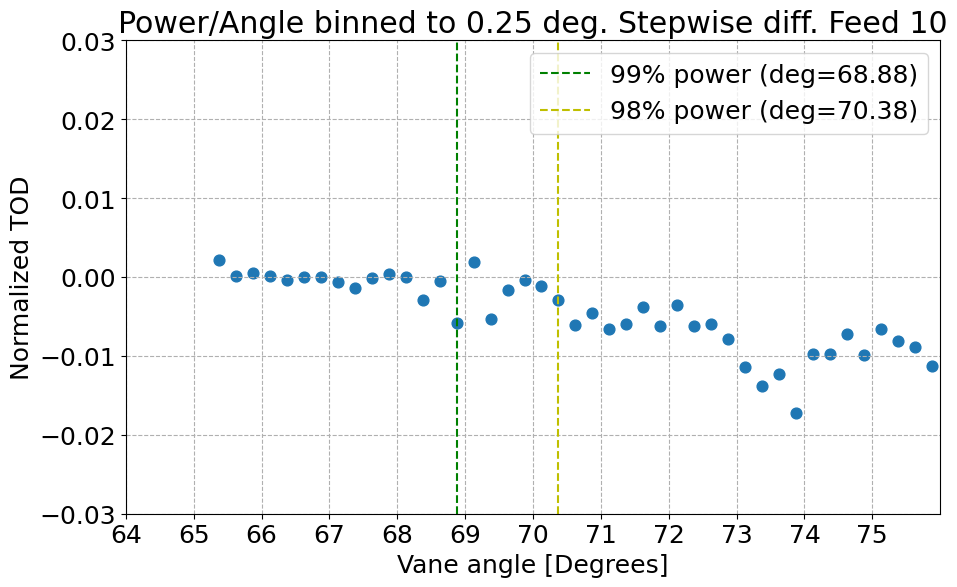
\includegraphics[scale=0.37]{../plots/binned_diff10.png}
    \caption{Difference from previous bin in 0.25 degree binned power/angle relation.}
    \label{fig:8and10_diff}
\end{figure}


\section{Angle drift and stuck vane occurrences}
As the cutoff angle seems to be in the neighborhood of 68 degrees, and the minimum angle obtained during a $T_{sys}$ measurement just barely passes this by a couple of degrees, it seemed worthwhile to look into if the minimum angle obtained has changed over time. If the health of the vane engine is declining, and it's drifting closer to 68 degrees over time, it would be a big problem.

Figure \ref{fig:angle_drift} contains the minimum vane angle obtained by each individual obsid over the 12 month span, categorized by month (left) and continually in time (right). The mean of each month, and a running gaussian window function, is also shown in each plot. While the plots doesn't point to a general drift, there instead seems to have been a transition where the average angle suddenly increased by $\sim 0.6$ degrees, from $65.5$ to $66.1$. This transition happens around MJD $58830$, obsid $9730$, or around the 13th of December 2019 (plus/minus a week or so).

\begin{figure}[H]
    \centering
    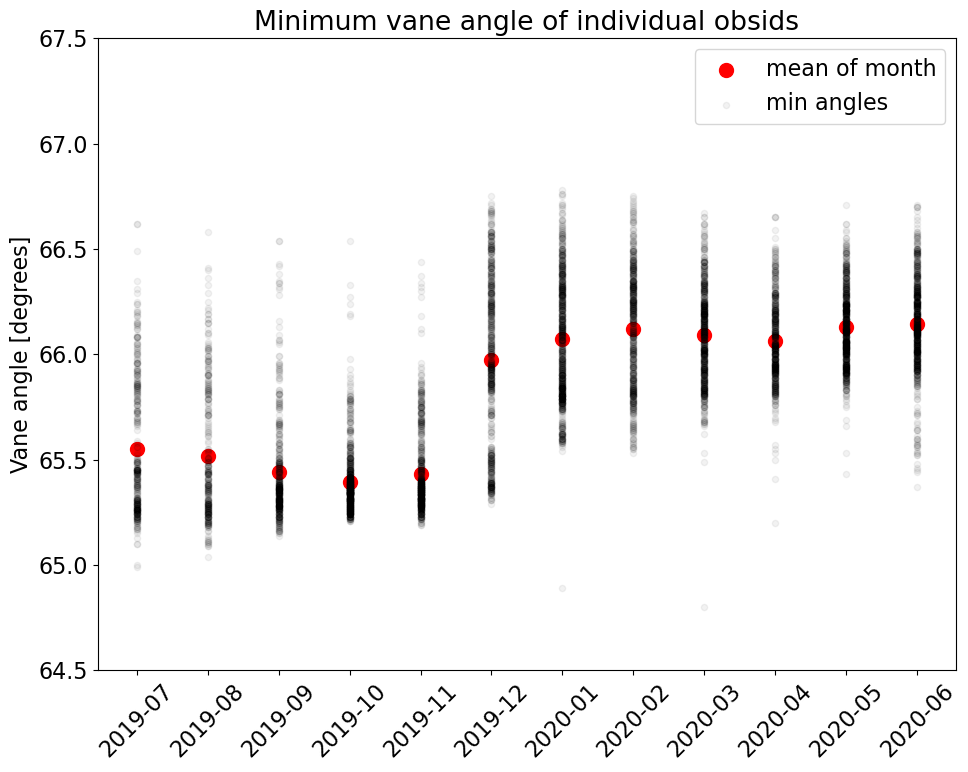
\includegraphics[scale=0.36]{../plots/angle_minima.png}
    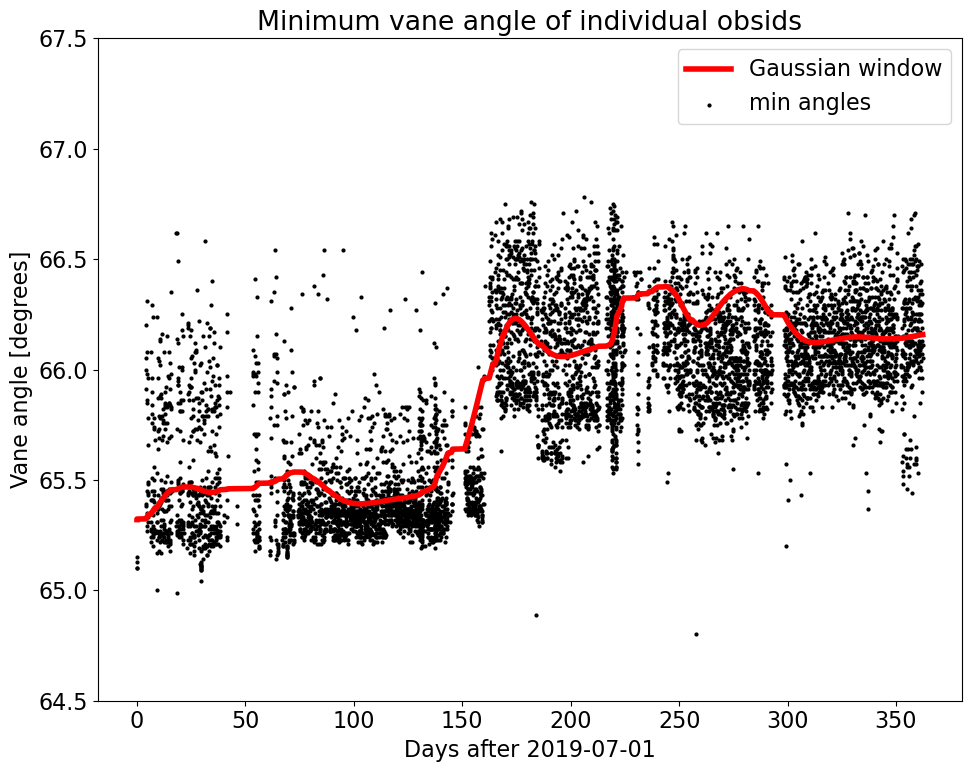
\includegraphics[scale=0.36]{../plots/angle_minima_datetime.png}
    \caption{Plots showing minimum angle obtained by the calibration vane for 12 months of level1 files, each point being a unique obsid. Left plot shows the monthly distribution of minimum angles, together with the average. Right plot shows the continuous distribution, with a Gaussian running window. Both plots clearly show a bump in minimum angle (as well as an increase in spread) around MJD $58830$, which is around the 13th of December, 2019.}
    \label{fig:angle_drift}
\end{figure}

Another related parameter of vane "health" is the frequency of which the vane was reported as "stuck". This can be gathered from the dataset \texttt{/hk/antenna0/vane/state}, where the state is set to $4$ for timesteps where the vane is reported as stuck. 

Figure \ref{fig:n_stuck} shows the number of stuck states in each obsid over 12 months of observation. We see a pretty substantial increase in stuck states from obsid 13000-13500 and onward. This is, interestingly, long after the sudden increase in minimum vane angle. There does appear to be a smaller increase in stuck vanes around the time of increased minimum angle (obsid ~9730), but it declines again very quickly.

\begin{figure}[H]
    \centering
    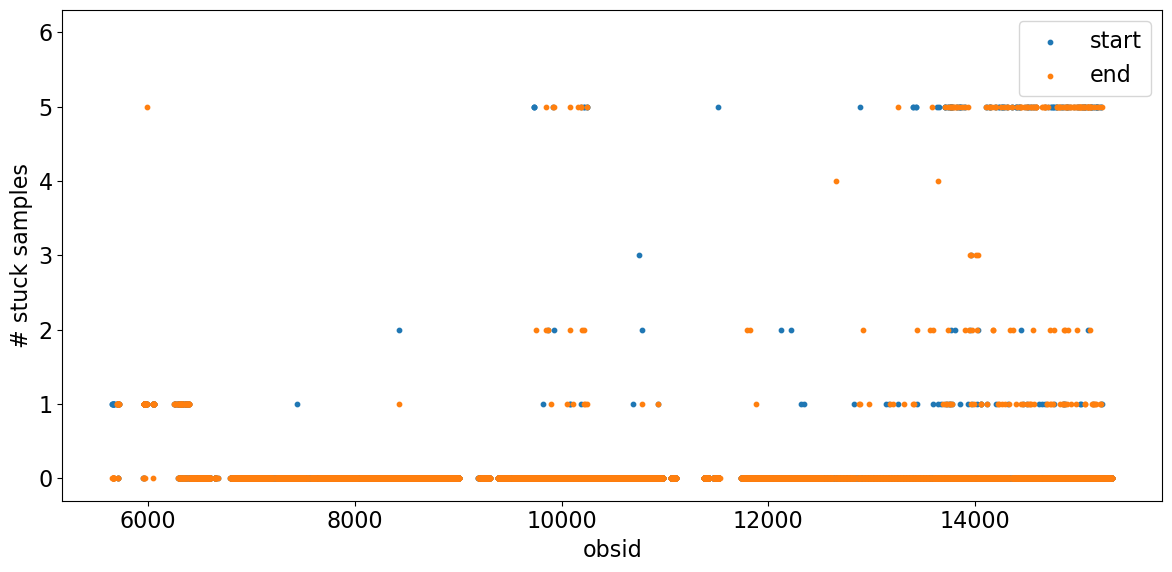
\includegraphics[scale=0.4]{../plots/n_stuck.png}
    \caption{Plot showing the number of times the vane was reported as stuck, during individual $T_{sys}$ measurements. The first and last $T_{sys}$ measurements in each obsid are shown individually.}
    \label{fig:n_stuck}
\end{figure}


\section{Conclusion}
An inconsistency between the timestamps of the spectrometer and timestamps of feed array was found. The offset strongly suggests a 0.6 second delay in the reported TOD power values of the spectrometer (or the feed array angles being 0.6 seconds ahead of time).

Accounting for this offset, feeds 8 and 10 were found to be the most sensitive to the calibration vane angle, and lose power the fastest as the angle increases. They both lost $1\%$ power as the vane increased to an angle of $68.88$ degrees, and a cutoff angle of $68$ degrees is recommended for any $T_{sys}$ measurement, to ensure that all feeds are sufficiently covered by the array.

There was also observed a sudden increase in the minimum angle obtainable by the calibration vane sometime around obsid 9730. The minimum obtainable angle suddenly increased from $\sim 65.5$ degrees to $\sim 66.1$ degrees. There did however not appear to be any continuous angle drift in time. Additionally, the frequency of stuck vane states have dramatically increased since obsid ca. 13000-13500 and onwards, although the lack of timing doesn't confirm this is directly linked to the change in minimum obtainable vane angle. 


\end{document}